\documentclass[10pt,aspectratio=169]{beamer}

\usepackage[utf8]{inputenc}
\usepackage[T1]{fontenc}
\usepackage{newtxtext,newtxmath}
\usepackage[english]{babel}
\usepackage{amsmath,amssymb,amsthm}
\usepackage{mathtools}
\usepackage{booktabs}
\usepackage{array}
\usepackage{graphicx}
\graphicspath{{assets/}}
\usepackage{tikz}
\usetikzlibrary{calc}
\usepackage{pgfplots}
\pgfplotsset{compat=1.18}
\usepackage{xcolor}
\usepackage{tcolorbox}
\tcbuselibrary{skins,breakable}

\usetheme{Madrid}
\usefonttheme{professionalfonts}
\usecolortheme{default}

\definecolor{parthenopenavy}{HTML}{1E2761}
\definecolor{parthenopeblue}{HTML}{2F3C7E}
\definecolor{parthenopeaccent}{HTML}{CADCFC}
\definecolor{highlightorange}{HTML}{D97706}

\setbeamercolor{structure}{fg=parthenopenavy}
\setbeamercolor{frametitle}{bg=parthenopenavy,fg=white}
\setbeamercolor{title}{fg=parthenopenavy}
\setbeamercolor{author}{fg=parthenopeblue}
\setbeamercolor{institute}{fg=parthenopeblue}

\setbeamerfont{frametitle}{series=\bfseries}
\setbeamertemplate{navigation symbols}{}

\setbeamertemplate{footline}{%
  \leavevmode%
  \hbox{%
  \begin{beamercolorbox}[wd=.4\paperwidth,ht=2.5ex,dp=1ex,leftskip=1em]{author in head/foot}%
    \usebeamerfont{author in head/foot}\underline{Feature-Driven Bias Detection}%
  \end{beamercolorbox}%
  \begin{beamercolorbox}[wd=.3\paperwidth,ht=2.5ex,dp=1ex,center]{title in head/foot}%
    \usebeamerfont{title in head/foot}A. Mungari%
  \end{beamercolorbox}%
  \begin{beamercolorbox}[wd=.3\paperwidth,ht=2.5ex,dp=1ex,rightskip=1em]{date in head/foot}%
    \hfill\usebeamerfont{date in head/foot}\insertframenumber{} / \inserttotalframenumber%
  \end{beamercolorbox}}%
  \vskip0pt%
}

\newtcolorbox{goalbox}[1][]{%
  colback=parthenopeaccent!30,
  colframe=parthenopenavy,
  fonttitle=\bfseries,
  title=Goal of the thesis,
  #1
}

\title[Feature-Driven Bias Detection]{Feature-Driven Bias Detection\\[2pt]
  \large An Association Rule Mining Approach\\to Analyze Feature Importance}
\author[A. Mungari]{Alfredo Mungari}
\institute[UniParthenope]{%
  University of Naples ``Parthenope''\\
  Department of Science and Technologies\\
  M.Sc.\ in Applied Computer Science --- Machine Learning \& Big Data\\[4pt]
  \emph{Master's Thesis}
}
\date{Academic Year 2024 / 2025}
\hypersetup{pdftitle={Feature-Driven Bias Detection}, pdfauthor={Alfredo Mungari}}

\begin{document}

% Slide 1
{\setbeamertemplate{footline}{}
\begin{frame}[plain]
  \begin{columns}[T,onlytextwidth]
    \begin{column}{0.18\textwidth}
      \raggedright
      
\includegraphics[height=1.8cm]{logo_uniparthenope.png}
    \end{column}
    \begin{column}{0.64\textwidth}
      \centering
      {\small\textbf{University of Naples ``Parthenope''}}\\[2pt]
      {\small Department of Science and Technologies}\\[2pt]
      {\small\itshape M.Sc.\ in Applied Computer Science --- Machine Learning \& Big Data}
    \end{column}
    \begin{column}{0.18\textwidth}
      \raggedleft
      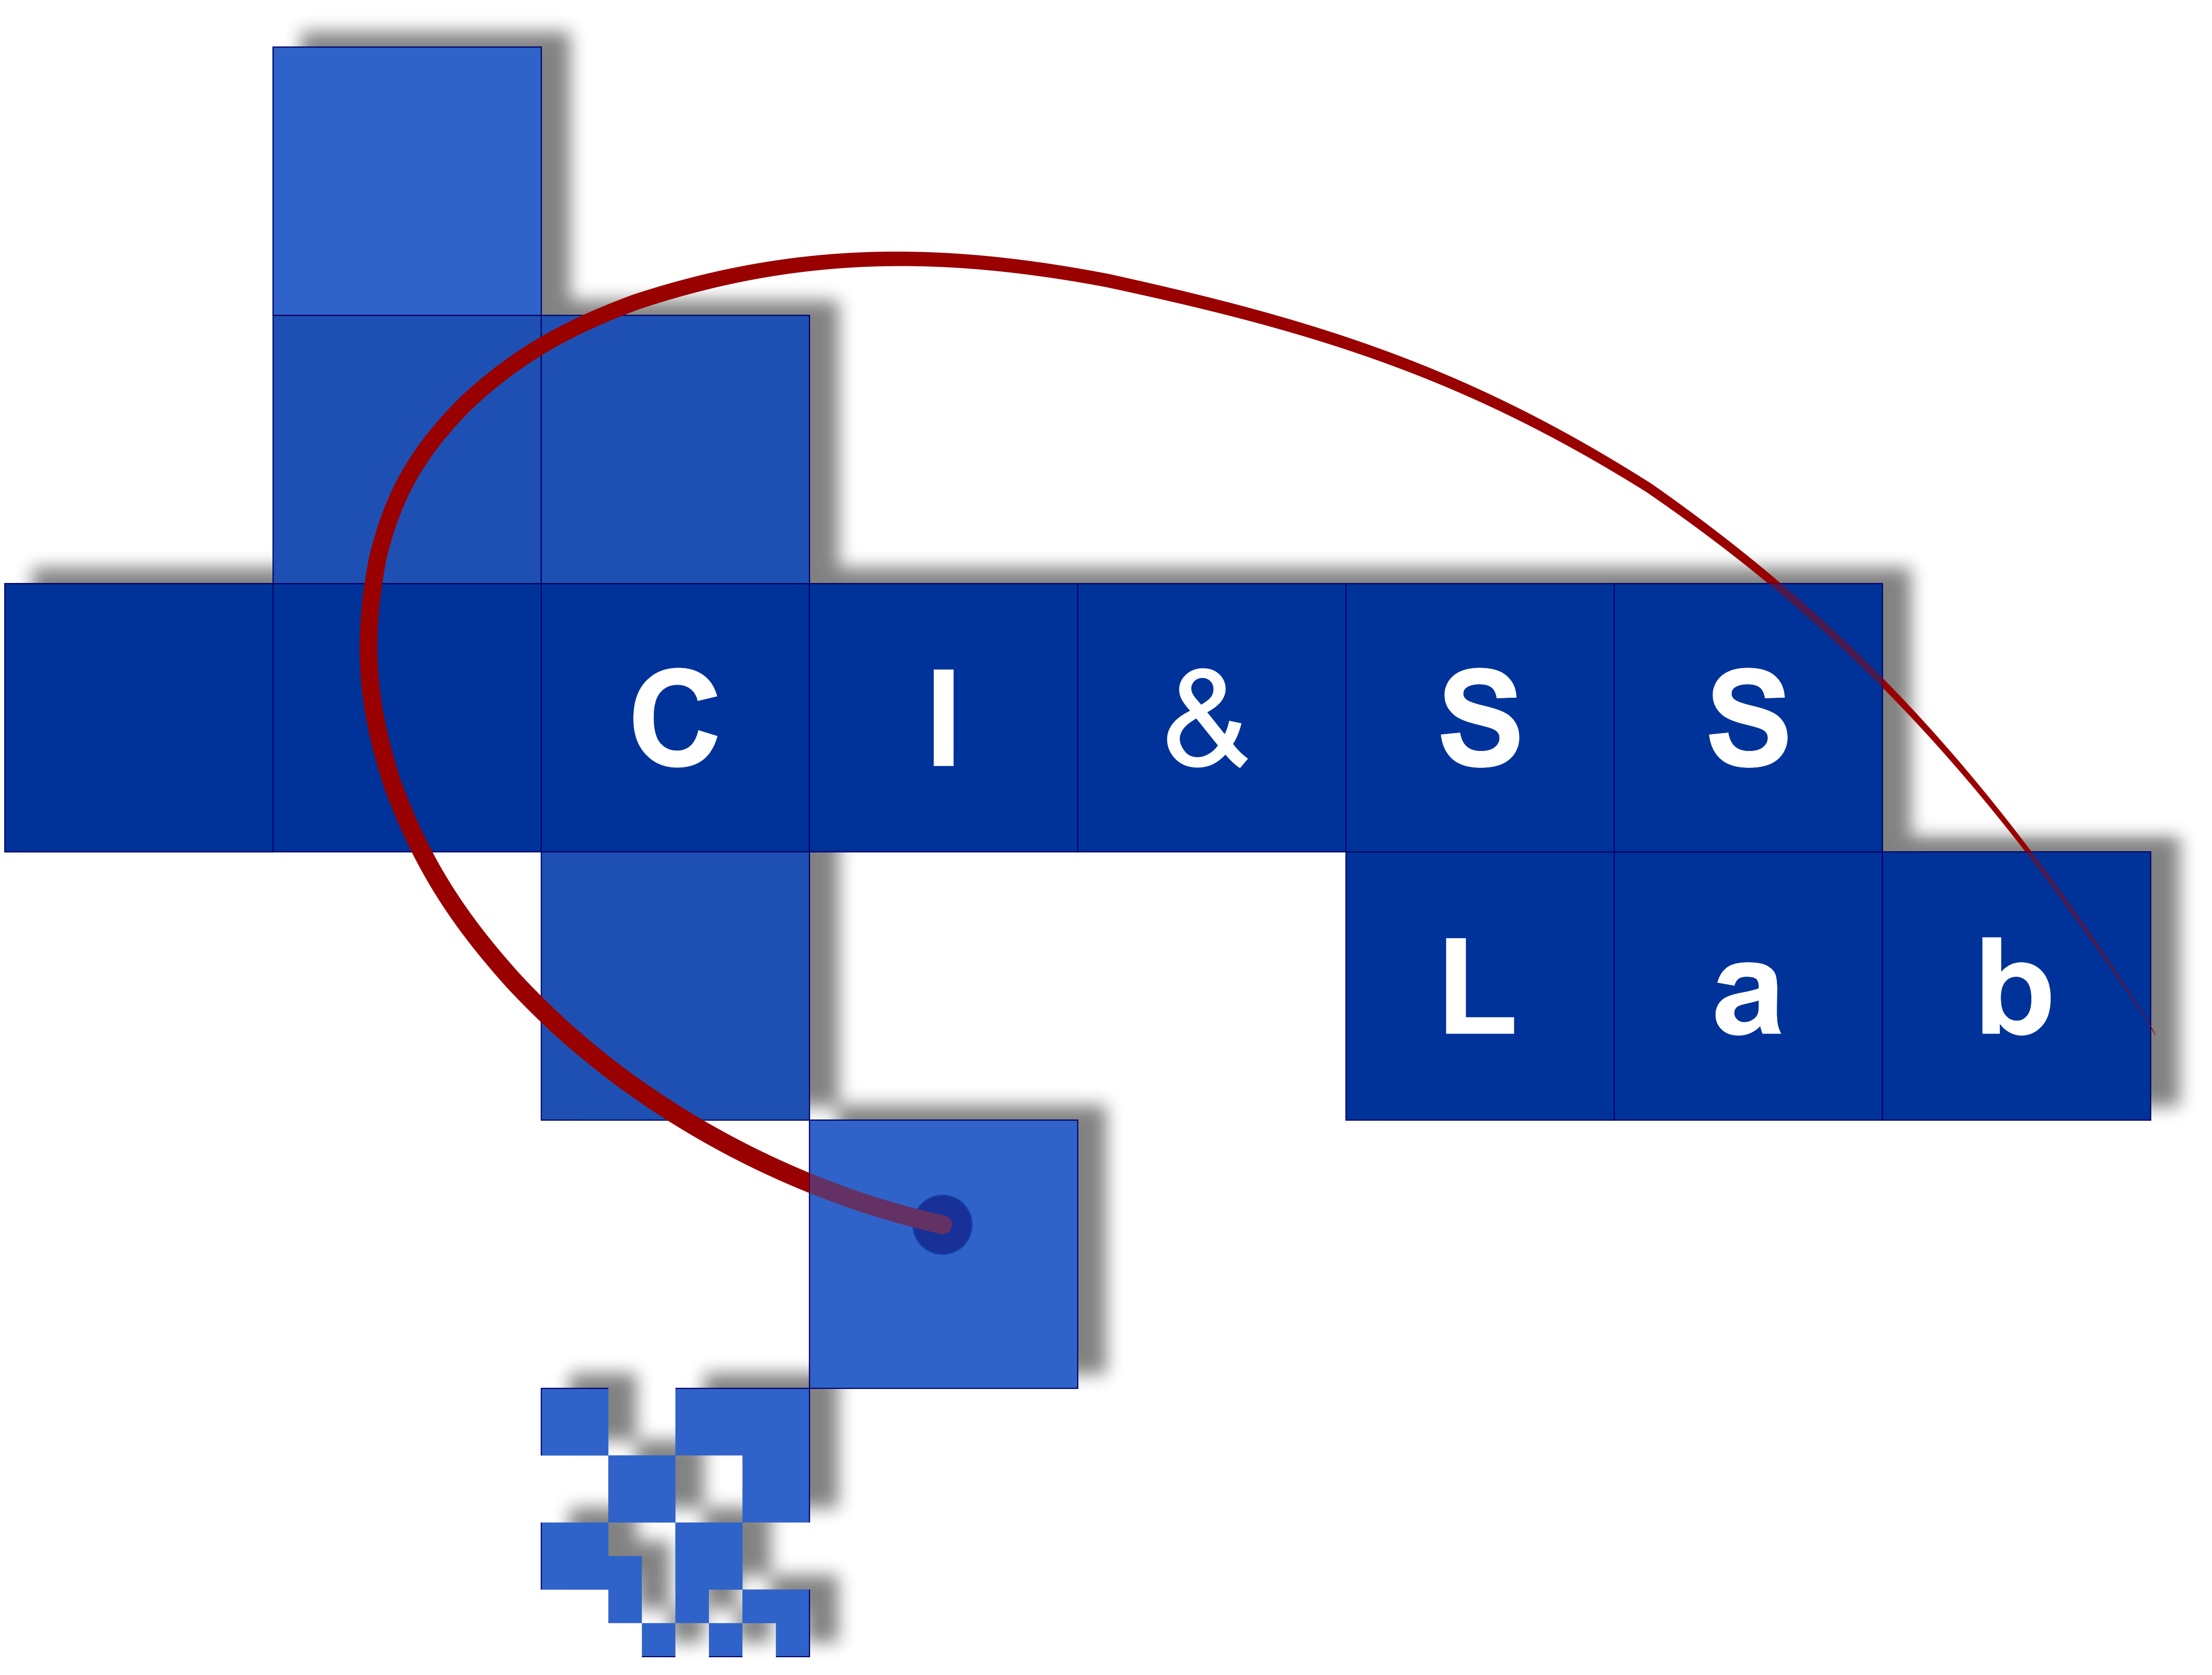
\includegraphics[height=1.8cm]{cisslab_logo.png}
    \end{column}
  \end{columns}
  \vspace{10pt}
  \begin{center}
    {\color{highlightorange}\small\textsc{Master's Thesis}}\\[10pt]
    {\color{parthenopenavy}\Huge\bfseries Feature-Driven Bias Detection}\\[6pt]
    {\color{parthenopenavy}\Large\itshape An Association Rule Mining Approach}\\[2pt]
    {\color{parthenopenavy}\Large\itshape to Analyze Feature Importance}
  \end{center}
  \vspace{10pt}
  \begin{columns}[T,onlytextwidth]
    \begin{column}{0.5\textwidth}
      \raggedright
      {\color{highlightorange}\scriptsize\textsc{Supervisor}}\\
      \textbf{Prof.\ Antonio Maratea}\\[8pt]
      {\color{highlightorange}\scriptsize\textsc{Examiner}}\\
      \textbf{Prof.\ Francesco Camastra}
    \end{column}
    \begin{column}{0.5\textwidth}
      \raggedleft
      {\color{highlightorange}\scriptsize\textsc{Candidate}}\\
      \textbf{Alfredo Mungari}\\
      {\small\itshape Student ID 0120000287}\\[8pt]
      {\small Academic Year 2024 / 2025}
    \end{column}
  \end{columns}
\end{frame}}

% Section 1 - Context and Motivations
\section{Context and Motivation}

{\setbeamertemplate{footline}{}
\begin{frame}[plain]
  \centering
  \vfill
  {\color{parthenopeblue}\large\textsc{Section 1}}\\[10pt]
  {\color{parthenopenavy}\Huge\bfseries Context and Motivation}
  \vfill
\end{frame}}

% Slide 3 
\begin{frame}{Explainable Artificial Intelligence (XAI) and Fairness}
  \begin{itemize}
    \item \textbf{XAI and the "Black-Box" Challenge}
    \begin{itemize}
        \item High-performing models (e.g., Deep Learning) are often \textbf{black boxes} due to their inherent \textbf{opacity}.
        \item XAI aims to make these decisions transparent, clarifying which factors influence a decision and how.
        \item Essential in high-stakes contexts: \textbf{credit}, \textbf{healthcare}, \textbf{hiring}, and \textbf{justice}.
    \end{itemize}
    
    \vspace{0.3cm}
    
    \item \textbf{Bias and Fairness}
    \begin{itemize}
        \item \textbf{The Bias Problem}: Systematic distortions or prejudices in data, collection procedures, or algorithms that lead to discriminatory outcomes.
        \item \textbf{Fairness}: The ethical principle and normative requirement of ensuring that decisions are impartial and equitable across different individuals or groups.
    \end{itemize}
  \end{itemize}
\end{frame}

% Slide 4
\begin{frame}{Counterfactual Explanations and Feature Importance}
  \begin{itemize}
    \item Given an instance $x_i$, its corresponding counterfactual $x_i^{CF}$ is an instance belonging to the opposite class $f(x_i^{CF}) \neq f(x_i)$ whose difference with respect to $x_i$ is minimal.
    \item Answers: \emph{``What was the minimum change to $x_i$ that would have led to a different decision?''}
    \item They are \textbf{local}, \textbf{model-agnostic} and \textbf{interpretable} explanations.
    \item According to recent literature, feature relevance can be measured based on counterfactuals: a feature is more relevant the more frequently its modification is required to flip the prediction (Alfeo et al., 2023).
  \end{itemize}
\end{frame}

% Slide 5
\begin{frame}{Association Rule Mining (ARM) and Thesis Goal}
  \begin{itemize}
    \item Born in \textbf{market basket analysis} (items bought together).
    \item A rule $A \Rightarrow B$ indicates that when $A$ occurs, $B$ is likely to occur too.
    \item \textbf{Our application}: items are the important features from counterfactuals. Extracted rules reveal the internal logic of the model.
  \end{itemize}
  \vspace{8pt}
  \begin{goalbox}
    Use ARM to identify the main decision patterns of the model from relevant features obtained through counterfactuals. In particular, we focus on rules containing \textbf{biased} and \textbf{actionable} attributes.
  \end{goalbox}
\end{frame}

% Section 2 - Methodology
\section{Methodology}

{\setbeamertemplate{footline}{}
\begin{frame}[plain]
  \centering
  \vfill
  {\color{parthenopeblue}\large\textsc{Section 2}}\\[10pt]
  {\color{parthenopenavy}\Huge\bfseries Methodology}
  \vfill
\end{frame}}

% Slide 7
\begin{frame}{Original BoCSoR Method (Alfeo et al., 2023)}
  \begin{columns}[T,onlytextwidth]
    \begin{column}{0.72\textwidth}
      \begin{itemize}\small
        \item \textbf{BoCSoR}: \emph{Boundary-based Counterfactual Scoring of Relevance} for tabular data.
        \item Designed for continuous spaces.
      \end{itemize}
      \textbf{Procedure:}
      \begin{enumerate}\small\setlength{\itemsep}{5pt}
        \item Compute for each $x_i$ the closest instance of the opposite class.
        \item Identify boundary instances: couples ``instance–closest opposite instance'' whose distance is less than a fixed percentile $p$.
        \item Compute 5 synthetic instances for each couple via linear interpolation, identifying as counterfactual $x_i^{CF}$ for $x_i$ the closest synthetic instance belonging to the opposite class.
        \item Perturbation step: substitute features $x_{ij}$ in $x_i^{CF}$ to check for a class change after re-classification, recording feature $j$ as relevant if the class changes.
        \item Compute BoCSoR score as global feature importance metric for each feature $j$.
      \end{enumerate}
    \end{column}
    \begin{column}{0.26\textwidth}
      \centering
      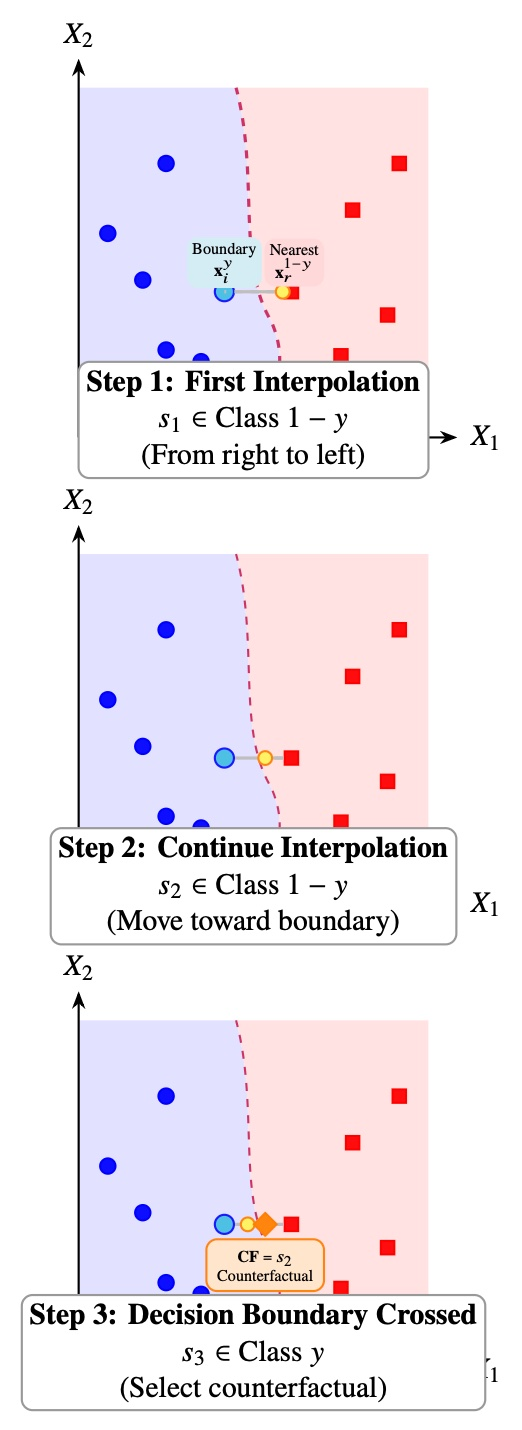
\includegraphics[height=6.9cm,keepaspectratio]{assets/fig_bocsor.png}
    \end{column}
  \end{columns}
\end{frame}

% Slide 8
\begin{frame}{Issues of BoCSoR for Categorical Data}
  Most real-world datasets contain tabular \textbf{categorical data}, especially in census data, where even quantitative numerical columns such as \emph{age} and \emph{hours worked} are organized into bands.
  \medskip

  The problems of adapting BoCSoR to categorical data are:
  \begin{itemize}
    \item Usage of Euclidean distance
    \item Interpolation step
  \end{itemize}
  In particular, in categorical cases features may be \textbf{categorical ordinal} or \textbf{categorical nominal}.
  \medskip

  \centering
  \footnotesize
  \begin{tabular}{@{}llllll@{}}
    \toprule
    AGEP & COW & SEX & SCHL & WKHP & \ldots \\
    \midrule
    Young & Emp.-Private-For-Profit & Female & Bachelors-Degree & Over-Full-time & \ldots \\
    Young-Adult & Emp.-Private-For-Profit & Female & Regular-HS-Diploma & Part-time & \ldots \\
    Retirement-Age & Local-Government-Employee & Male   & Masters-Degree & Full-time & \ldots \\
    \ldots & \ldots & \ldots & \ldots & \ldots & \ldots \\
    \bottomrule
  \end{tabular}
\end{frame}

% Slide 9
\begin{frame}{Hybrid Encoding and Unified Distance}
  \begin{itemize}\small
    \item Before explaining BoCSoR adaptation to categorical case, it is necessary to define how nominal and ordinal data are encoded and processed.
    \item Categorical space: $\tilde{x}_i = (x_i^{nom}, x_i^{ord}) \in \tilde{\mathcal{X}}$
    \item Each feature $X_j$ is encoded to represent each possible categorical value assigned to it $c_{jk} \in C_j$, introducing new features for each instance: $enc(\tilde{x}_{ij}) = c_{jk}$
    \item \textbf{Encoding strategy}:
      \begin{itemize}
        \item \textbf{Nominal}: \emph{one-hot encoding} (scaled by 0.5) in $\{0, 1\}$.
        \item \textbf{Ordinal}: \emph{rank encoding} + \emph{min-max scaling} in $[0, 1]$.
      \end{itemize}
    \item \textbf{A single distance}: the distance between two instances is the global Manhattan distance, defined as the sum of the Manhattan distances across the individual encoded features, ensuring coherence between heterogeneous types:
  \end{itemize}
  \begin{equation*}
    d_{man}(\tilde{x}_a, \tilde{x}_b) = \sum_j d_{man}\bigl(enc(\tilde{x}_{aj}),\, enc(\tilde{x}_{bj})\bigr)
  \end{equation*}
\end{frame}

% Slide 10
\begin{frame}{Examples of Ordinal and Nominal Encoding}
  \scriptsize
  \begin{columns}[T,onlytextwidth]
    \begin{column}{0.49\textwidth}
      \textbf{Example (ordinal only).} Consider two instances $\tilde{\mathbf{x}}_a$ and $\tilde{\mathbf{x}}_b$ on the same $j$-th ordinal feature, with four ordered categories $(c_{j1} \prec c_{j2} \prec c_{j3} \prec c_{j4})$ and $p_j = 4$. Suppose that $x^{\mathrm{ord}}_{aj} = c_{j2}$ and $x^{\mathrm{ord}}_{bj} = c_{j4}$.
      \begin{equation*}
        \mathrm{rank}(x^{\mathrm{ord}}_{aj}) = 2,\qquad \mathrm{rank}(x^{\mathrm{ord}}_{bj}) = 4
      \end{equation*}
      After min-max normalization,
      \begin{equation*}
        \mathrm{ord\_enc}(x^{\mathrm{ord}}_{aj}) = \frac{2-1}{4-1} = \frac{1}{3},\qquad
        \mathrm{ord\_enc}(x^{\mathrm{ord}}_{bj}) = \frac{4-1}{4-1} = 1
      \end{equation*}
      The Manhattan distance on this ordinal feature is
      \begin{equation*}
        d_{\mathrm{Man}}\!\left(\mathrm{ord\_enc}(x^{\mathrm{ord}}_{aj}),\mathrm{ord\_enc}(x^{\mathrm{ord}}_{bj})\right)
        = \left|\frac{1}{3}-1\right| = \frac{2}{3}
      \end{equation*}
      Hence, each ordinal-feature contribution lies in $[0,1]$.
    \end{column}
    \begin{column}{0.49\textwidth}
      \textbf{Example (nominal only).} Let $\mathcal{C}_j = \{c_1,c_2,c_3\}$ and consider two instances $\tilde{\mathbf{x}}_a$ and $\tilde{\mathbf{x}}_b$ such that $x^{\mathrm{nom}}_{aj} = c_1$ and $x^{\mathrm{nom}}_{bj} = c_3$.
      \begin{equation*}
        \mathrm{one\_hot}(x^{\mathrm{nom}}_{aj}) = (1,0,0),\qquad
        \mathrm{one\_hot}(x^{\mathrm{nom}}_{bj}) = (0,0,1)
      \end{equation*}
      The Manhattan distance on this unscaled block is
      \begin{equation*}
        d_{\mathrm{Man}}\!\left(\mathrm{one\_hot}(x^{\mathrm{nom}}_{aj}),\mathrm{one\_hot}(x^{\mathrm{nom}}_{bj})\right) = 2
      \end{equation*}
      After scaling by $1/2$,
      \begin{equation*}
        \mathrm{nom\_enc}(x^{\mathrm{nom}}_{aj}) = (0.5,0,0),\qquad
        \mathrm{nom\_enc}(x^{\mathrm{nom}}_{bj}) = (0,0,0.5)
      \end{equation*}
      Evaluating the Manhattan distance on these scaled encodings yields
      \begin{equation*}
        d_{\mathrm{Man}}\!\left(\mathrm{nom\_enc}(x^{\mathrm{nom}}_{aj}),\mathrm{nom\_enc}(x^{\mathrm{nom}}_{bj})\right) = 1
      \end{equation*}
      Hence, each nominal-feature distance contribution is within $\{0,1\}$.
    \end{column}
  \end{columns}
\end{frame}

% Slide 11
\begin{frame}{Adaptation to the Categorical Case}
  \begin{columns}[T,onlytextwidth]
    \begin{column}{0.54\textwidth}
      The space $\tilde{\mathcal{X}}$ is \textbf{categorical}:
      \begin{itemize}\scriptsize
        \item Euclidean $\rightarrow$ \textbf{Global Manhattan} distance.
        \item Linear interpolation $\rightarrow$ \textbf{$k$-nearest opposite-class neighbors} for each categorical instance $\tilde{x}_i$, since in a categorical space perturbing the closest counterfactual cannot be enough to flip the class label.
        \item Perturbation step records a list of relevant \textcolor{highlightorange}{feature = category pair} $X_j = c_{jk}$ for each instance across all $k$-counterfactuals:
        {\scriptsize
        \begin{equation*}
          L_i = \bigcup_{r=1}^{k}\bigl\{(X_j = c_{jk}) \,\big|\, j \in \{1, \ldots, n_{cat}\},\; f(\tilde{x}_{i,r}^{CF,j}) = f(\tilde{x}_i)\bigr\}
        \end{equation*}
        }
        \item Store $\mathcal{E}$ the set of all $L_i$ for each $\tilde{x}_i$, considered as a transactional database.
      \end{itemize}
    \end{column}
    \begin{column}{0.44\textwidth}
      \centering
      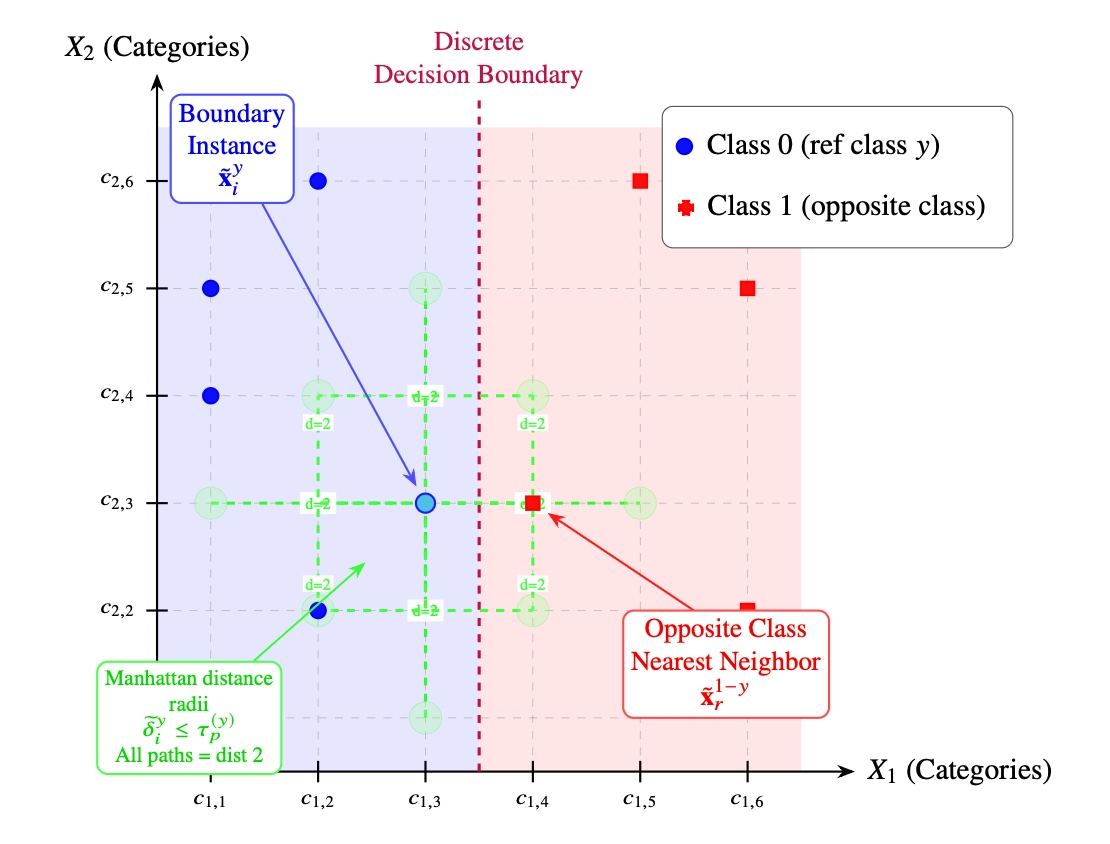
\includegraphics[width=\textwidth,keepaspectratio]{assets/fig_categorical.png}
    \end{column}
  \end{columns}
\end{frame}

% Slide 12
\begin{frame}{ARM in the Thesis Context}
  \begin{itemize}\small
    \item \textbf{Input Data}: ARM operates on the lists of relevant features ($L_i$) extracted in the previous step.
    \item \textbf{Feature Space}: these lists belong to the transaction database $\mathcal{E}$.
    \item \textbf{Transaction Representation}: each instance is modeled as a transaction of its specific relevant features.
  \end{itemize}
  \vspace{4pt}
  
  \begin{tcolorbox}[colback=parthenopeaccent!20,colframe=parthenopenavy,boxrule=0.5pt,arc=1pt]
    \begin{columns}[T,onlytextwidth]
      \begin{column}{0.48\textwidth}
        \textbf{Classic ARM (Market Basket)}\\[2pt]
        \footnotesize
        List of items: \{Milk, Bread, Butter, \ldots\}\\[4pt]
        $x_1 = \{ \text{Milk, Cereal, Butter} \}$\\
        $x_2 = \{ \text{Bread, Milk} \}$\\
        $x_3 = \{ \text{Butter, Eggs, Flour} \}$
      \end{column}
      \begin{column}{0.48\textwidth}
        \textbf{Our Proposed Case}\\[2pt]
        \footnotesize
        Items = relevant feature--category pairs extracted from counterfactuals.\\[4pt]
        $x_1 = \{ f_3, f_6, f_8 \}$\\
        $x_2 = \{ f_1, f_3 \}$\\
        $x_3 = \{ f_2, f_8, f_{10} \}$
      \end{column}
    \end{columns}
  \end{tcolorbox}
  
  \vspace{4pt}
  \textbf{Example Rule Comparison:}
  \begin{itemize}\small
    \item \textbf{Classic Market Basket}: \{\text{Butter}\} $\Rightarrow$ \{\text{Milk}\}
    \item \textbf{Feature-Based Case}: $\{f_1\} \Rightarrow \{f_3\}$
  \end{itemize}
\end{frame}

\begin{frame}{ARM Metrics: Evaluating Feature Associations}
  \textbf{Goal:} Quantifying the strength and reliability of the extracted rules $X \Rightarrow Y$ (e.g., $f_1 \Rightarrow f_3$). Let $N$ be the total number of samples.
  \vspace{10pt}

  \begin{itemize}\small
    \item \textbf{Support}: Measures the frequency of the pattern. How often do features $X$ and $Y$ appear together as relevant in the dataset?
    $$ \text{Support}(X \Rightarrow Y) = \frac{\text{freq}(X \cup Y)}{N} $$
    \vspace{2pt}

    \item \textbf{Confidence}: Measures the reliability of the inference (conditional probability). If feature $X$ is relevant, how likely is it that $Y$ is also relevant?
    $$ \text{Confidence}(X \Rightarrow Y) = \frac{\text{Support}(X \cup Y)}{\text{Support}(X)} $$
    \vspace{2pt}

    \item \textbf{Lift}: Measures the strenght of correlation of the association compared to random chance.
    $$ \text{Lift}(X \Rightarrow Y) = \frac{\text{Support}(X \cup Y)}{\text{Support}(X) \times \text{Support}(Y)} $$
    
    \vspace{4pt}
    {\footnotesize
    $\text{Lift} > 1$: positive association \hfill
    $\text{Lift} = 1$: independence \hfill
    $\text{Lift} < 1$: negative association.
    }
  \end{itemize}
\end{frame}

% Hierarchical ARM overview
\begin{frame}{Hierarchical ARM: Why Two Levels?}
  Applying ARM directly to $\mathcal{E}$ raises two issues:
  \begin{itemize}\small
    \item \textbf{Combinatorial explosion}: with $n_{cat}$ features and up to $p_j$ categories each, the rule space grows as $\bigl(\sum_j p_j\bigr)^k$ for itemsets of size $k$.
    \item \textbf{Interpretive fragmentation}: rules like $\{\mathrm{SCHL{=}Bachelors}\} \Rightarrow \{\mathrm{OCCP{=}Tech}\}$ and $\{\mathrm{SCHL{=}Masters}\} \Rightarrow \{\mathrm{OCCP{=}Prof}\}$ are reported as independent, yet both instantiate the same coarser pattern: \textsc{Schl} and \textsc{Occp} tend to be jointly relevant.
  \end{itemize}
  \vspace{4pt}
  \begin{tcolorbox}[colback=parthenopeaccent!25,colframe=parthenopenavy,boxrule=0.5pt,arc=1pt]
    \textbf{Solution:} organize the analysis into \emph{two levels of granularity}.
    \begin{columns}[T,onlytextwidth]
      \begin{column}{0.48\textwidth}
        \small\textbf{Macroscopic level} --- \emph{features only}:\\
        \textcolor{highlightorange}{which features} are jointly relevant?\\[2pt]
        Example: $\{\mathrm{SCHL}\} \Rightarrow \{\mathrm{OCCP}\}$
      \end{column}
      \begin{column}{0.48\textwidth}
        \small\textbf{Microscopic level} --- \emph{feature = category pairs}:\\
        \textcolor{highlightorange}{which categorical combinations} realize each macro rule?\\[2pt]
        Example: $\{\mathrm{SCHL{=}Bach.}\} \Rightarrow \{\mathrm{OCCP{=}Tech}\}$
      \end{column}
    \end{columns}
  \end{tcolorbox}
\end{frame}

% Macroscopic analysis
\begin{frame}{Macroscopic Analysis}
  \textbf{Projection onto feature names.} For each local explanation $\mathcal{L}_i \in \mathcal{E}$, keep only the feature indices, discarding the categories:
  \begin{equation*}
    \mathcal{M}_i = \{\, X_j \mid (X_j = c_{jk}) \in \mathcal{L}_i \,\}, 
    \qquad \mathcal{M} = \{\mathcal{M}_i \mid \mathcal{L}_i \in \mathcal{E}\}.
  \end{equation*}
  \textbf{Mining.} Run ARM on $\mathcal{M}$ to obtain candidate rules $A_{\mathrm{macro}} \Rightarrow B_{\mathrm{macro}}$ between \emph{feature names}.
  \vspace{4pt}
  
  \begin{tcolorbox}[colback=parthenopeaccent!25,colframe=parthenopenavy,boxrule=0.5pt,arc=1pt,title=\bfseries Filtering thresholds (macroscopic)]
    \small
    A candidate rule is kept in $\mathcal{R}_{\mathrm{macro}}$ if and only if:
    \begin{itemize}\small
      \item $\mathrm{supp}(R) \geq \tau_{\mathrm{supp}}^{\mathrm{macro}}$ \quad (frequent across boundary instances)
      \item $\mathrm{conf}(R) \geq \tau_{\mathrm{conf}}^{\mathrm{macro}}$ \quad (reliable implication)
      \item $\mathrm{lift}(R) \notin [1 - \epsilon,\, 1 + \epsilon]$ \quad (non-independence: discard chance co-occurrence)
    \end{itemize}
  \end{tcolorbox}
  \vspace{2pt}
  \textbf{Output.} The set $\mathcal{R}_{\mathrm{macro}}$ of \emph{structural dependencies} between features, e.g.:\\
  \quad $\{\mathrm{SCHL}\} \Rightarrow \{\mathrm{OCCP}\}, \quad \{\mathrm{SCHL}, \mathrm{AGEP}\} \Rightarrow \{\mathrm{OCCP}\}$.
\end{frame}

% Microscopic analysis
\begin{frame}{Microscopic Analysis}
  \textbf{Per-rule restriction.} For each macro rule $R \in \mathcal{R}_{\mathrm{macro}}$, consider only the transactions in $\mathcal{E}$ that contain a category for \emph{every} feature of $R$:
  \begin{equation*}
    \mathcal{E}_R = \{\, \mathcal{L}_i \in \mathcal{E} \mid \forall X_j \in A_{\mathrm{macro}} \cup B_{\mathrm{macro}},\ \exists\, (X_j = c_{jk}) \in \mathcal{L}_i \,\}.
  \end{equation*}
  Running ARM on $\mathcal{E}_R$ yields rules $A_{\mathrm{micro}} \Rightarrow B_{\mathrm{micro}}$ on \textcolor{highlightorange}{feature = category pairs}, each being a specialization of $R$.
  \vspace{4pt}
  
  \begin{tcolorbox}[colback=parthenopeaccent!25,colframe=parthenopenavy,boxrule=0.5pt,arc=1pt,title=\bfseries Filtering thresholds (microscopic)]
    \scriptsize
    Within $\mathcal{E}_R$, support is bounded by $|\mathcal{E}_R| \ll |\mathcal{E}|$ and is split across categories: lower thresholds are required.
    \begin{itemize}\small
      \item $\mathrm{supp}(r) \geq \tau_{\mathrm{supp}}^{\mathrm{micro}}$, \ with $\tau_{\mathrm{supp}}^{\mathrm{micro}} < \tau_{\mathrm{supp}}^{\mathrm{macro}}$
      \item $\mathrm{conf}(r) \geq \tau_{\mathrm{conf}}^{\mathrm{micro}}$, \ with $\tau_{\mathrm{conf}}^{\mathrm{micro}} < \tau_{\mathrm{conf}}^{\mathrm{macro}}$
      \item $\mathrm{lift}(r) \notin [1 - \epsilon,\, 1 + \epsilon]$ \ (same independence window)
    \end{itemize}
  \end{tcolorbox}
  \vspace{2pt}
  \textbf{Output.} A mapping $\mathcal{R}_{\mathrm{micro}} : R \mapsto \mathcal{R}_{\mathrm{micro}}(R)$ that attaches to each macro rule its category-level specializations. Example for $\{\mathrm{SCHL}\} \Rightarrow \{\mathrm{OCCP}\}$:\\
  \quad $\{\mathrm{SCHL{=}Bachelors}\} \Rightarrow \{\mathrm{OCCP{=}Tech\text{-}support}\}$.
\end{frame}

% section 3 - Dataset and Data Preparation
\section{Dataset and Data Preparation}

{\setbeamertemplate{footline}{}
\begin{frame}[plain]
  \centering
  \vfill
  {\color{parthenopeblue}\large\textsc{Section 3}}\\[10pt]
  {\color{parthenopenavy}\Huge\bfseries Dataset and Data Preparation}
  \vfill
\end{frame}}

% slide 15
\begin{frame}{Limitations of Classic Tabular Benchmarks}
  \begin{itemize}
    \item In Fairness/XAI literature, recurring benchmarks like \textbf{Adult}, \textbf{COMPAS}, and \textbf{German Credit} are standard.
    \item While useful for methodological comparisons, they have \textbf{limited empirical coverage}: small sample sizes, dated historical contexts, and low heterogeneity.
    \item They often exhibit \textbf{weak anonymization}, \textbf{hidden proxies}, and \textbf{weak documentation}, leading to reduced semantic richness.
    \item Issues like \textbf{missing values}, \textbf{encoding artifacts}, and \textbf{preprocessing errors} can bias both model performance and fairness assessments.
  \end{itemize}
\end{frame}

% slide 16
\begin{frame}{From UCI Adults to Folktables}
  \textbf{The Adult problem} (Ding et al., 2021), standard de facto for census data:
  \begin{itemize}\small
    \item Data from the 1994 CPS; the fixed \$50{,}000 threshold is no longer socio-economically meaningful.
    \item $< 50k$ records $\cdot$ 14 features $\cdot$ no geographic stratification.
    \item Coding artifacts (\texttt{fnlwgt}, a demographic weight) often misused as predictive features.
    \item Weak anonymization and hidden proxies limit semantic richness.
  \end{itemize}
  \medskip
  \textbf{The solution: Folktables} (Ding et al., 2021)
  \begin{itemize}\small
    \item Recent ACS PUMS microdata from the US Census Bureau.
    \item Reproducible and configurable by year, task and geography.
    \item Focus task: \textbf{ACSIncome} (binary income classification).
    \item Key advantage: bias varies across socio-economic contexts.
  \end{itemize}
\end{frame}

% slide 17
\begin{frame}{Data Preparation and Augmentation}
  \centering
  \small
  \begin{tabular}{@{}lllll@{}}
    \toprule
    \textbf{Benchmark} & \textbf{Size} & \textbf{Records} & \textbf{Threshold $\theta$} & \textbf{Socio-Economic Profile} \\
    \midrule
    NY Metropolitan Area   & Small  & 106,877   & \$94{,}400   & Urbanized and rich \\
    Texas                  & Small  & 145,670   & \$90{,}800   & Poor and rural \\
    Northeast              & Medium & 508,138   & \$100{,}700  & Urbanized and rich \\
    South                  & Medium & 642,617   & \$86{,}000   & Poor and rural \\
    ALL (U.S.\ except AK)  & Large  & 1,753,049 & \$94{,}200   & Highly heterogeneous (National baseline) \\
    \bottomrule
  \end{tabular}
\end{frame}

% section 3 - Results
\section{Results}

{\setbeamertemplate{footline}{}
\begin{frame}[plain]
  \centering
  \vfill
  {\color{parthenopeblue}\large\textsc{Section 4}}\\[10pt]
  {\color{parthenopenavy}\Huge\bfseries Results}
  \vfill
\end{frame}}

% slide 19
\begin{frame}{Experimental Setup and Semantic Classification}
  \begin{columns}[T,onlytextwidth]
    \begin{column}{0.48\textwidth}
      \textbf{Setup (320 configurations)}
      \begin{itemize}\small
        \item \textbf{Data source}: ACS \textbf{2024}.
        \item \textbf{5 geographic benchmarks}: NY, TX, Northeast, South, ALL.
        \item \textbf{2 models}: CatBoost (axis-aligned splits), MLP (smooth surfaces).
        \item \textbf{8 neighborhood sizes}:\\ $k \in \{1, 3, 5, 7, 9, 11, 13, 15\}$.
        \item \textbf{4 boundary percentiles}:\\ $P \in \{10, 15, 20, 25\}\%$.
        \item \textbf{Rule thresholds}: different values of support and confidence were evaluated via grid search, while a fixed lift window width of \textbf{25} was used.
      \end{itemize}
    \end{column}
    \begin{column}{0.48\textwidth}
      \textbf{Rule Classification}
      \begin{itemize}\small
        \item \textbf{Actionable}: only modifiable features (SCHL, COW, WKHP, OCCP).
        \item \textbf{Biased}: contains at least one sensitive feature (SEX, RAC1P).
        \item \textbf{Other}: contextual (AGEP, MAR, RELP, POBP).
        
      \end{itemize}
    \end{column}
  \end{columns}
\end{frame}

% slide 20
\begin{frame}{Macroscopic Results: Geographic Asymmetry}
  \begin{columns}[T,onlytextwidth]
    \begin{column}{0.62\textwidth}
      \centering
      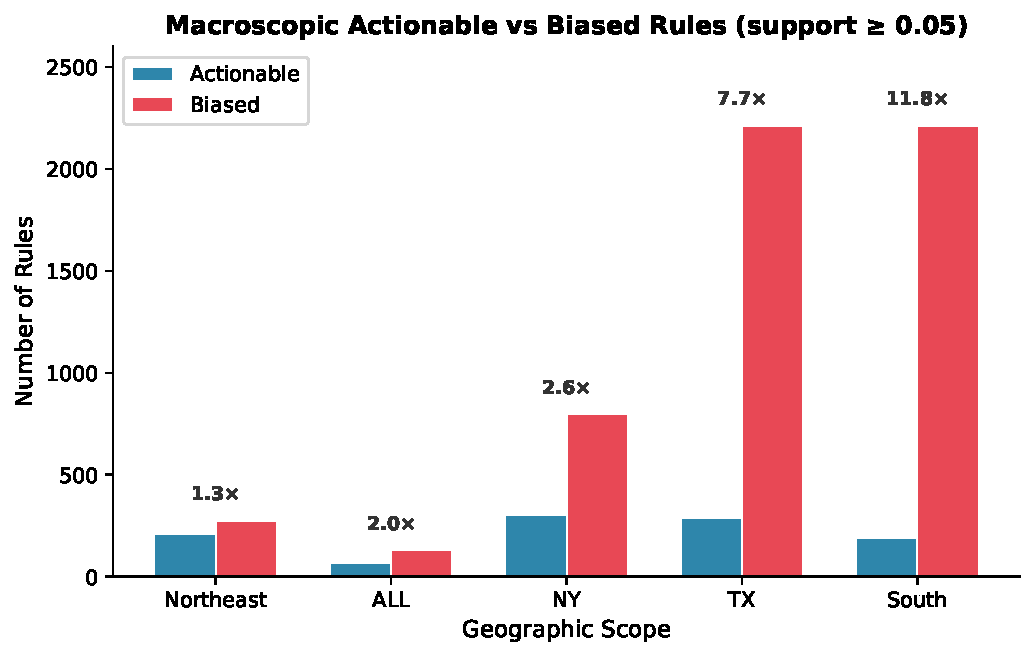
\includegraphics[width=\textwidth,keepaspectratio]{fig_actionable_vs_biased.pdf}
    \end{column}
    \begin{column}{0.36\textwidth}
      \small
      \begin{itemize}
        \item Dominant \textbf{actionable}:\\ \textcolor{highlightorange}{COW $\Rightarrow$ OCCP}.
        \item Dominant \textbf{biased}:\\ \textcolor{highlightorange}{RAC1P $\Rightarrow$ OCCP}.
        \item \textbf{South}: unique pattern\\ \textcolor{highlightorange}{RAC1P $\Rightarrow$ POBP}\\(Race–Birthplace proxy).
        \item Biased/Actionable ratio:\\ \textbf{11.8$\times$} in the South vs \textbf{1.3$\times$} in NE.
      \end{itemize}
    \end{column}
  \end{columns}
\end{frame}

% slide 21
\begin{frame}{Decay Analysis: Which Rules Persist?}
  \begin{columns}[T,onlytextwidth]
    \begin{column}{0.66\textwidth}
      \centering
      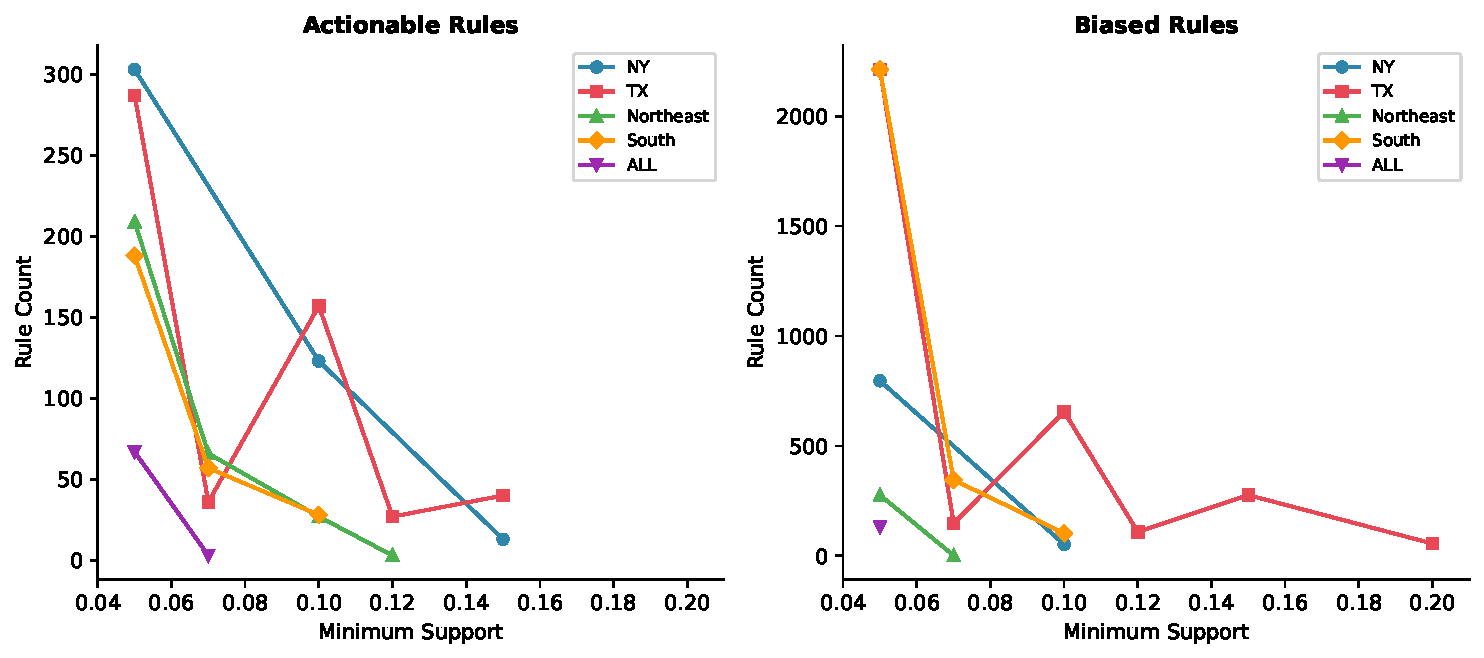
\includegraphics[width=\textwidth,keepaspectratio]{fig_decay.pdf}
    \end{column}
    \begin{column}{0.32\textwidth}
      \small
      \begin{itemize}
        \item \textbf{NE \& NY}: actionable rules persist at higher support levels.
        \item \textbf{TX \& South}: biased rules are extremely robust (up to supp $\geq 0.20$).
        \item \textbf{National data (ALL)} dilutes local bias patterns.
      \end{itemize}
    \end{column}
  \end{columns}
\end{frame}

% slide 22
\begin{frame}{Microscopic Results: Profiling the Bias}
  \begin{itemize}\setlength{\itemsep}{10pt}
    \item \textbf{Texas -- Gender bias in education:}\\
      \quad $\{\mathrm{COW{=}Local\text{-}Gov},\ \mathrm{SEX{=}Female}\} \Rightarrow \{\mathrm{OCCP{=}Education}\}$
    \item \textbf{New York -- Occupational segmentation:}\\
      \quad $\{\mathrm{RAC1P{=}White},\ \mathrm{SEX{=}Female}\} \Rightarrow \{\mathrm{OCCP{=}Office\text{-}Admin}\}$
    \item \textbf{South -- Geography as racial proxy:}\\
      \quad $\{\mathrm{RAC1P{=}Black}\} \Rightarrow \{\mathrm{POBP{=}Georgia}\}$
  \end{itemize}
\end{frame}

% section 5 - Conclusions
\section{Conclusions}

{\setbeamertemplate{footline}{}
\begin{frame}[plain]
  \centering
  \vfill
  {\color{parthenopeblue}\large\textsc{Section 5}}\\[10pt]
  {\color{parthenopenavy}\Huge\bfseries Conclusions}
  \vfill
\end{frame}}

% slide 24
\begin{frame}{Conclusions and Future Work}
  \textbf{Main Findings}
  \begin{itemize}
    \item ARM + Counterfactuals is effective for global XAI and bias detection.
    \item Identified clear geographic asymmetries in ML model prediction.
    \item Hierarchical design is key to understanding the ``how'' and ``why'' of decison pattern.
  \end{itemize}
  \bigskip
  \textbf{Future Work}
  \begin{itemize}
    \item Temporal analysis (fairness drift).
    \item Integration with Causal Inference.
    \item Evaluation on other types of classifiers.
  \end{itemize}
\end{frame}

% slide 25
{\setbeamertemplate{footline}{}
\begin{frame}[plain]
  \centering
  \vfill
  {\color{parthenopenavy}\Huge\bfseries Thank you for your attention}\\[20pt]
  {\color{parthenopeblue}\large Alfredo Mungari}\\[4pt]
  {\color{parthenopeblue}\normalsize UniParthenope --- 2024/2025}
  \vfill
\end{frame}}

\end{document}